\documentclass[11pt]{article}
% -------------------------------
% Shared packages and commands
% -------------------------------

% --- Page size & margins ---
\usepackage[a4paper,top=2cm,bottom=2.5cm,left=2cm,right=2cm]{geometry}

% --- Title formatting ---
\usepackage{titling}

% Move the whole title block up
\setlength{\droptitle}{-2em}

% Keep author and date on their own lines, just reduce the gaps
\pretitle{\begin{center}\LARGE\bfseries}%
\posttitle{\par\end{center}\vspace{-0.5em}} % space after title
\preauthor{\begin{center}\large}%
\postauthor{\par\end{center}\vspace{-0.5em}} % space after author
\predate{\begin{center}\small}%
\postdate{\par\end{center}\vspace{-1em}} % space after date block


% --- Math & theorem environments ---
\usepackage{amsmath, amssymb, amsthm}

% --- Graphics & tables ---
\usepackage{graphicx}
\usepackage{booktabs}

% --- Hyperlinks ---
\usepackage{hyperref}
\hypersetup{
  colorlinks=true,
  linkcolor=blue,
  urlcolor=blue
}

% --- Optional: underlined hyperlinks (remove if not desired) ---
% \usepackage[normalem]{ulem}
% \renewcommand\UrlFont{\uline}

% --- Custom macros (add your own below) ---
% \newcommand{\R}{\mathbb{R}}

\title{SPC707P Machine and Deep Learning — Week 02 Project}
\author{Kavit Tolia} 
\date{\today}

\usepackage{fancyhdr}
\usepackage{lastpage}

\begin{document}
\maketitle

\pagestyle{fancy}
\fancyhf{}%
\fancyfoot[C]{\thepage\ of \pageref{LastPage}}

% Make the 'plain' style (used on first page, after \maketitle, etc.) match:
\fancypagestyle{plain}{%
  \fancyhf{}%
  \fancyfoot[C]{\thepage\ of \pageref{LastPage}}
  \renewcommand{\headrulewidth}{0pt}
  \renewcommand{\footrulewidth}{0pt}
}

\section{Exercise 1}
Write an expression to calculate the variance of \texttt{my\_array} and compare it to \texttt{np.var(my\_array)}. First, let's recall the definition of the variance:
\[
 \dfrac{1}{N} \sum_{i=1}^{N} (x_i - \overline{x})^2
\]
One can notice that this is basically the mean of the array $(x_i - \overline{x})^2$. You can do this in 4 steps:
\begin{enumerate}
    \item Write an expression for the mean of \texttt{my\_array}
    \item Define a new array as the difference between \texttt{my\_array} and its mean
    \item Square your new array
    \item Calculate the mean of \texttt{new\_array\_squared}. Compare this to the variance calculated with \texttt{numpy}.
\end{enumerate}
\textit{Solution.} 
\begin{lstlisting}
import numpy as np
my_array = np.array([10, 15, 15, 20, 25, 30, 32])
arr_mean = np.sum(my_array) / my_array.size
new_array = my_array - arr_mean
new_array_squared = new_array ** 2
my_array_var = np.sum(new_array_squared) / new_array_squared.size
print(f"My calculated variance = {my_array_var:.2f}, using numpy we get {np.var(my_array):.2f}")
\end{lstlisting}
\textit{Output:} \texttt{My calculated variance = 58.86, using numpy we get 58.86}

\section{Exercise 2}
Write an expression to find the mode of \texttt{my\_array}. \\
\textit{Solution.}
\begin{lstlisting}
import numpy as np
my_array = np.array([10, 15, 15, 20, 25, 30, 32])
unique_arr = np.unique(my_array)
freq_arr = np.zeros(unique_arr.size)
for idx, val in enumerate(unique_arr):
    freq_arr[idx] = np.sum(my_array == val)
max_freq = np.max(freq_arr)
my_mode = unique_arr[freq_arr == max_freq]
if len(my_mode) == 1:
    print(f"The mode of my_array is {my_mode[0]}")
else:
    print(f"The modes of my_array are {my_mode}")
\end{lstlisting}
\textit{Output:} \texttt{The mode of my\_array is 15}

\section{Exercise 3}
\begin{enumerate}
    \item Define a simple function to greet someone (use default values for arguments).
    \item Call the function without any input to verify that the default values work.
    \item Call the function with different inputs to verify that the function works as expected.
    \item Define another function that determines whether a number is even or odd.
    \item Call the function and store the result, then print the result.
    \item Define a function that calls the first two functions and greets someone and displays whether their age is even or odd.
\end{enumerate}
\textit{Solution.}
\begin{lstlisting}
def say_hello(output='Hello World!'):
    print(output)

say_hello()
say_hello('Now say this!')

def even_or_odd(num):
    if (num % 2 == 0):
        return 'even'
    else:
        return 'odd'

test_num = 3
result = even_or_odd(test_num)
print(f"The number {test_num} is {result}.")

def greet_person(age, greeting='Hello World!'):
    say_hello(greeting)
    print(f"Your age is {even_or_odd(age)}")

greet_person(4)
\end{lstlisting}
\textit{Output:} \\
\texttt{
Hello World! \\
Now say this! \\
The number 3 is odd. \\
Hello World! \\
Your age is even \\
}

\section{Exercise 4}
The purpose of this exercise is to get you to play around with \texttt{pandas} \texttt{DataFrame} and to consolidate the knowledge that you already have.
\begin{itemize}
    \item Generate 5 samples with 100{,}000 correlated random numbers distributed according to Gaussian distributions (you can choose whatever covariance matrix you like, although you can start with an identity matrix for simplicity). You may want to use the \texttt{numpy} function \texttt{random.multivariate\_normal} for this purpose.
    \item Read these into a DataFrame.
    \item Create a 6\textsuperscript{th} column in your DataFrame: the values should be the second column plus the fourth column.
    \item Verify that the covariance (and correlation) matrices are what you would expect.
    \item Display your data.
\end{itemize}
\textit{Solution.}
\begin{lstlisting}
import numpy as np
import pandas as pd
num_var = 5
means = np.zeros(num_var)
cov_matrix = np.identity(num_var)
num_samples = 100000
col_names = ['Var1', 'Var2', 'Var3', 'Var4', 'Var5']
random_multivariate = np.random.multivariate_normal(means, cov_matrix, num_samples)
df = pd.DataFrame(random_multivariate, columns=col_names)
df = df.assign(
    Var6 = df['Var2'] + df['Var4']
)
print("The covariances are what we expect within sampling error. The variance of Var6 is 2 which is correct as it's the sum of 1 and 1")
display(df.cov(numeric_only=True))
display(df.head())
\end{lstlisting}
\textit{Output:}
\texttt{The covariances are what we expect within sampling error. The variance of Var6 is 2 which is correct as it's the sum of 1 and 1}
\begin{figure}[h!]
  \centering
  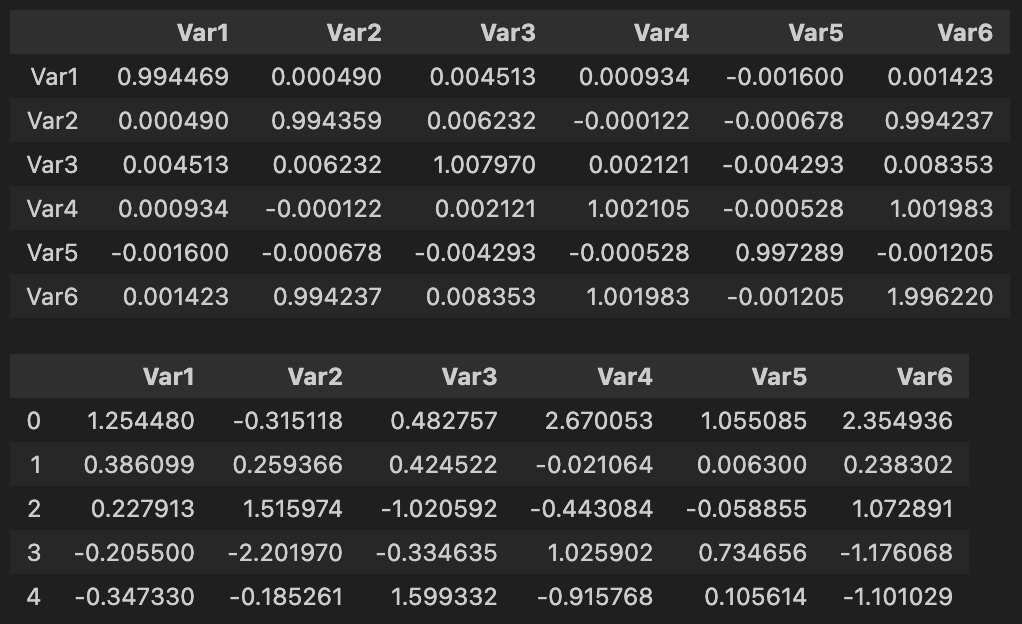
\includegraphics[width=\textwidth]{../exercise_4_output.png}
\end{figure}

\section{Exercise 5}
Let's analyse some data from the euro/dollar and pound/dollar exchange rates.
\begin{enumerate}
    \item Read the euro--dollar exchange rate file into a DataFrame and merge it with the pound--dollar DataFrame. You may want to use the \texttt{pandas} \texttt{rename} function to rename the columns.
    \item Check the dataset for \texttt{NaN} and drop any instances of \texttt{NaN}.
    \item Plot histograms and time series from the DataFrame.
    \item Calculate mean, variance, covariance, and correlation.
    \item Plot a scatter plot of the euro--dollar vs.\ the pound--dollar exchange. You may notice the graph showing two separate populations. Use the slice function to try to separate the two populations \emph{(hint: the ideal index will be between 2000 and 3000)}.
    \item Calculate the coefficients for the linear regression \(y = mx + q\) for the three samples (the total sample, and the two samples found with the split in point~5), and plot them on top of a scatter graph:
    \[
        m = \dfrac{\sigma_{xy}}{\sigma_x^2}
    \]
    \[
        q = \overline{y}-m\overline{x}
    \]
    You may want to use \texttt{stats.linregress} from \texttt{scipy} to calculate the coefficients.
    \item Write a sentence of your interpretation of the graph.
\end{enumerate}
\textit{Solution.}
\begin{enumerate}
    \item 
    \leavevmode
      \begin{lstlisting}
      import pandas as pd
      import numpy as np
      import matplotlib.pyplot as plt
      from scipy import stats
      df_eur = pd.read_csv('data/euro-dollar-exchange-rate-historical-chart.csv')
      df_gbp = pd.read_csv('data/pound-dollar-exchange-rate-historical-chart.csv')
      df = pd.merge(df_eur, df_gbp, on='date')
      df.rename(columns={' value_x': 'eurusd', ' value_y': 'gbpusd'}, inplace=True)
      df.set_index('date', inplace=True)
      df.head()
      \end{lstlisting}
    \item 
    \leavevmode
      \begin{lstlisting}
      df.info() # No NaNs found from this!
      <class 'pandas.core.frame.DataFrame'>
      Index: 6257 entries, 1999-01-04 to 2022-09-23
      Data columns (total 2 columns):
      #   Column  Non-Null Count  Dtype  
      ---  ------  --------------  -----  
      0   eurusd  6257 non-null   float64
      1   gbpusd  6257 non-null   float64
      dtypes: float64(2)
      memory usage: 146.6+ KB
      \end{lstlisting}
    \item 
    \leavevmode
      \begin{lstlisting}
      df.hist()
      df.plot(rot=45)
      \end{lstlisting}

    \vfill
    \begin{center}
        \textit{Figure shown on next page $\rightarrow$}
    \end{center}
    \newpage

    \noindent
    \begin{minipage}[t]{0.48\textwidth}
        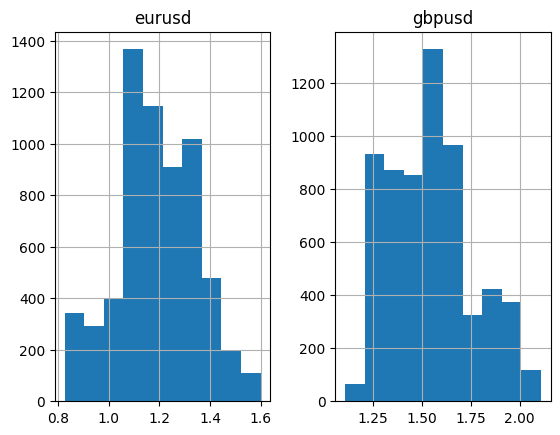
\includegraphics[width=\textwidth]{../exercise_5_hist.png}
    \end{minipage}%
    \hfill
    \begin{minipage}[t]{0.48\textwidth}
        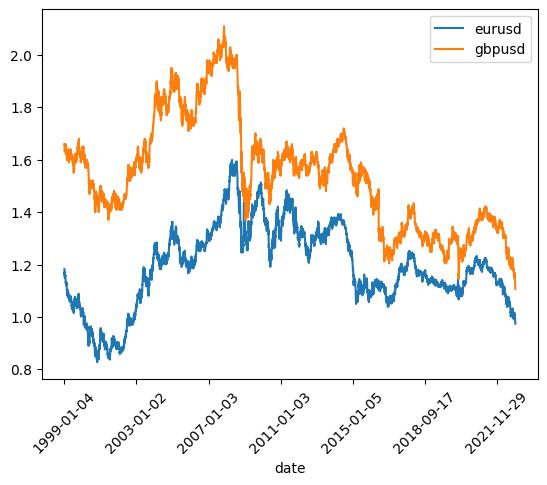
\includegraphics[width=\textwidth]{../exercise_5_ts.png}
    \end{minipage}

    \item 
    \leavevmode
      \begin{lstlisting}
      summary = pd.DataFrame({
          'mean': df.mean(),
          'std': df.std()
      })
      for col in df.columns:
          summary[f"corr_{col}"] = df.corr()[col]
          summary[f"cov_{col}"] = df.cov()[col]
      summary
      \end{lstlisting}
      \begin{figure}[h!]
        \centering
        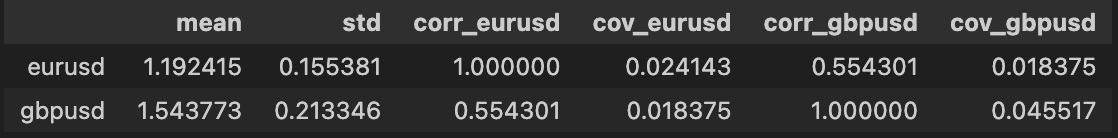
\includegraphics[width=\textwidth]{../exercise_5_metrics.png}
      \end{figure}

    \item 
    \leavevmode
      \begin{lstlisting}
      plt.scatter(df['eurusd'], df['gbpusd'])
      plt.xlabel('eurusd')
      plt.ylabel('gbpusd')
      \end{lstlisting}
    \vfill
    \begin{center}
        \textit{Figure shown on next page $\rightarrow$}
    \end{center}
    \newpage
      \begin{figure}[h!]
        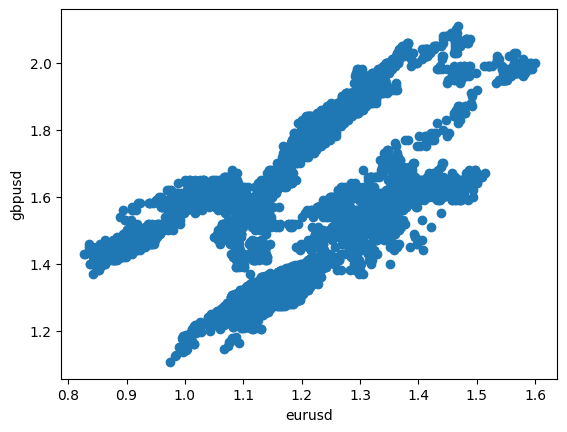
\includegraphics[width=\textwidth]{../exercise_5_scatter_all.png}
      \end{figure}
      \begin{lstlisting}
      row_slice = slice(2300, df.shape[0])
      post_df = df.iloc[row_slice]
      pre_df = df.iloc[:row_slice.start]
      plt.scatter(pre_df['eurusd'], pre_df['gbpusd'])
      plt.scatter(post_df['eurusd'], post_df['gbpusd'])
      plt.xlabel('eurusd')
      plt.ylabel('gbpusd')
      \end{lstlisting}
      \vfill
      \begin{center}
          \textit{Figure shown on next page $\rightarrow$}
      \end{center}
      \newpage
      \begin{figure}[h!]
        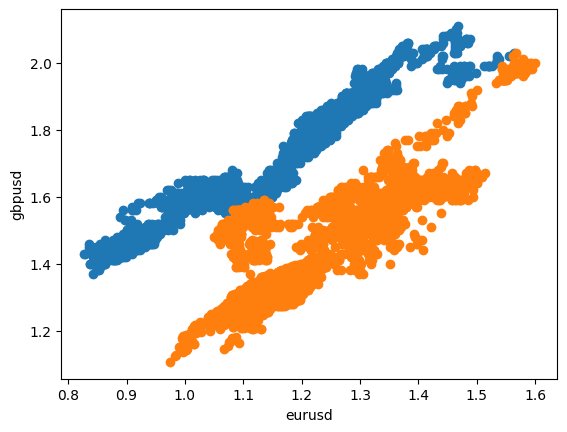
\includegraphics[width=\textwidth]{../exercise_5_scatter_split.png}
      \end{figure}

    \item 
    \leavevmode
      \begin{lstlisting}
      datasets = {
          "all": df,
          "pre": pre_df,
          "post": post_df
      }
      colors = {
          "all": "gray",
          "pre": "blue",
          "post": "green"
      }
      plt.figure(figsize=(8,6))
      for label, d in datasets.items():
          x = d["eurusd"]
          y = d["gbpusd"]
          plt.scatter(x, y, alpha=0.4, label=f"{label} data", color=colors[label])
          res = stats.linregress(x, y)
          x_fit = np.linspace(x.min(), x.max(), 100)
          y_fit = res.intercept + res.slope * x_fit
          plt.plot(x_fit, y_fit, color=colors[label], lw=2,
                  label=f"{label} fit (slope={res.slope:.2f})")
      plt.xlabel("eurusd")
      plt.ylabel("gbpusd")
      plt.legend()
      plt.show()
      \end{lstlisting}
      \vfill
      \begin{center}
          \textit{Figure shown on next page $\rightarrow$}
      \end{center}
      \newpage
      \begin{figure}[h!]
        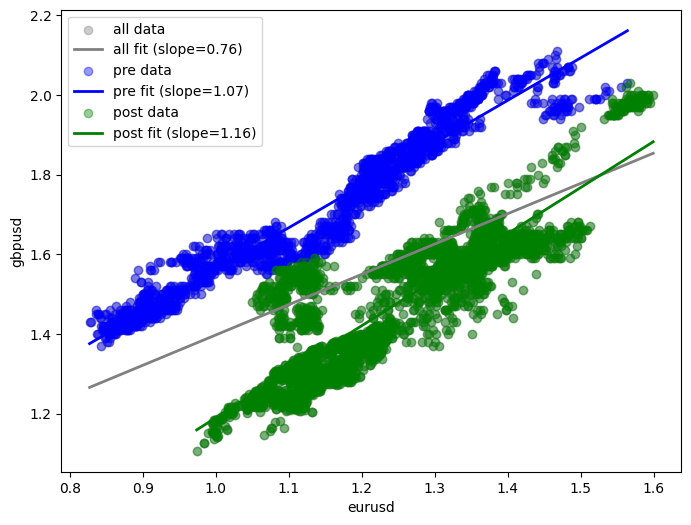
\includegraphics[width=\textwidth]{../exercise_5_scatter_linreg.png}
      \end{figure}

      \item There seems to be two different regimes (pre-2008 and post-2008), where the behaviour 
            of the the variables seems to change somewhat. This makes it clear how important the 
            data window is in any time series analysis. You could also say that a linear regression 
            done using either pre-2008 or post-2008 data would provide a higher $R^2$ compared to the 
            $R^2$ for the entire period. 
\end{enumerate}

\end{document}